\documentclass[border=4pt]{standalone}
% Preámbulo común de las figuras. Cada figura es un documento standalone
% que se compila a SVG con scripts/build_figures.sh
\usepackage[utf8]{inputenc}
\usepackage{amsmath}
\usepackage{tikz}
\usepackage[american, siunitx]{circuitikz}
\usetikzlibrary{arrows.meta,calc,decorations.pathmorphing,patterns}
\tikzset{
  >={Stealth[length=2.2mm]},
  eje/.style={->, thin},
  hilo/.style={thick},
}
% Paleta común: tonos medios legibles sobre fondo claro
\definecolor{azul}{RGB}{31,94,168}
\definecolor{rojo}{RGB}{192,57,43}
\definecolor{verde}{RGB}{39,128,73}
\definecolor{naranja}{RGB}{211,120,30}
\definecolor{morado}{RGB}{125,60,152}

\begin{document}
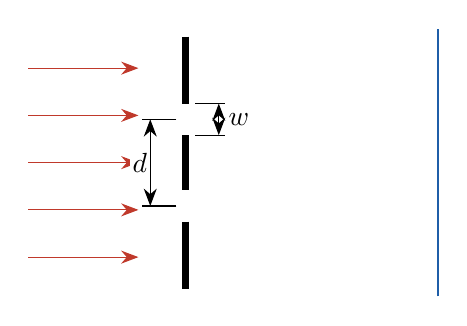
\begin{tikzpicture}[scale=1.0]
  \foreach \y in {-1.2,-0.6,0,0.6,1.2} \draw[->, rojo] (-2.0,\y) -- (-0.6,\y);
  \draw[line width=2.4pt] (0,1.6) -- (0,0.75);
  \draw[line width=2.4pt] (0,0.35) -- (0,-0.35);
  \draw[line width=2.4pt] (0,-0.75) -- (0,-1.6);
  \draw[thin] (0.12,0.75) -- (0.5,0.75); \draw[thin] (0.12,0.35) -- (0.5,0.35);
  \draw[<->] (0.42,0.75) -- node[right]{$w$} (0.42,0.35);
  \draw[thin] (-0.12,0.55) -- (-0.55,0.55); \draw[thin] (-0.12,-0.55) -- (-0.55,-0.55);
  \draw[<->] (-0.45,0.55) -- node[left, fill=white, inner sep=1pt]{$d$} (-0.45,-0.55);
  \draw[thick, azul] (3.2,-1.7) -- (3.2,1.7);
\end{tikzpicture}
\end{document}
